%!TEX root = ../main.tex

\chapter{Softwarearkitektur}

\RevisionsTabel{Software Arkitektur}{
		& 	 	&   \\
		& 		&   \\
		& 		&   \\
		& 	 	&   \\
}

I dette afsnit beskrives softwarearkitekturen for AVS\fxnote{AVS glossary}, som der er blevet givet indblik på i systemarkitekturen. Afsnittet skulle gerne give et indblik på det specificeret software indenfor fastlagte ramme, så udviklerne evt. kunne udarbejde det. Afsnittet indeholder dokumentation og design af de forskellige softwaredele med test på nogle af dem. \\
I afsnittet er softwaren delt ud i fire forskellige blokke som er delt op ud fra domain modelen. De fire blokke er GUI, FlexPMS, KarControl og \gls{sensoroe}. 

%!TEX root = ../../main.tex

\section{Design og implementering af database og GUI}
I dette afsnit kommer vi ind på beskrivelsen af databasen og \glslink{gui}{GUI'ens} design og implementering. Der vil være en beskrivelse af hvordan disse er anvendt i systemmet og hvordan de løser de problematikker der er stillet i kravspecifikationen.\\

\subsection{GUI}
Som udgangspunkt til at lave \glslink{gui}{GUI'en} er der blevet implementeret en webside, hvor selve kommunikation mellem databasen, websiden, clienten mm. ser ud som det kan ses i diagrammet på figur \ref{fig:web}.

\begin{figure}[H]
    \centering
    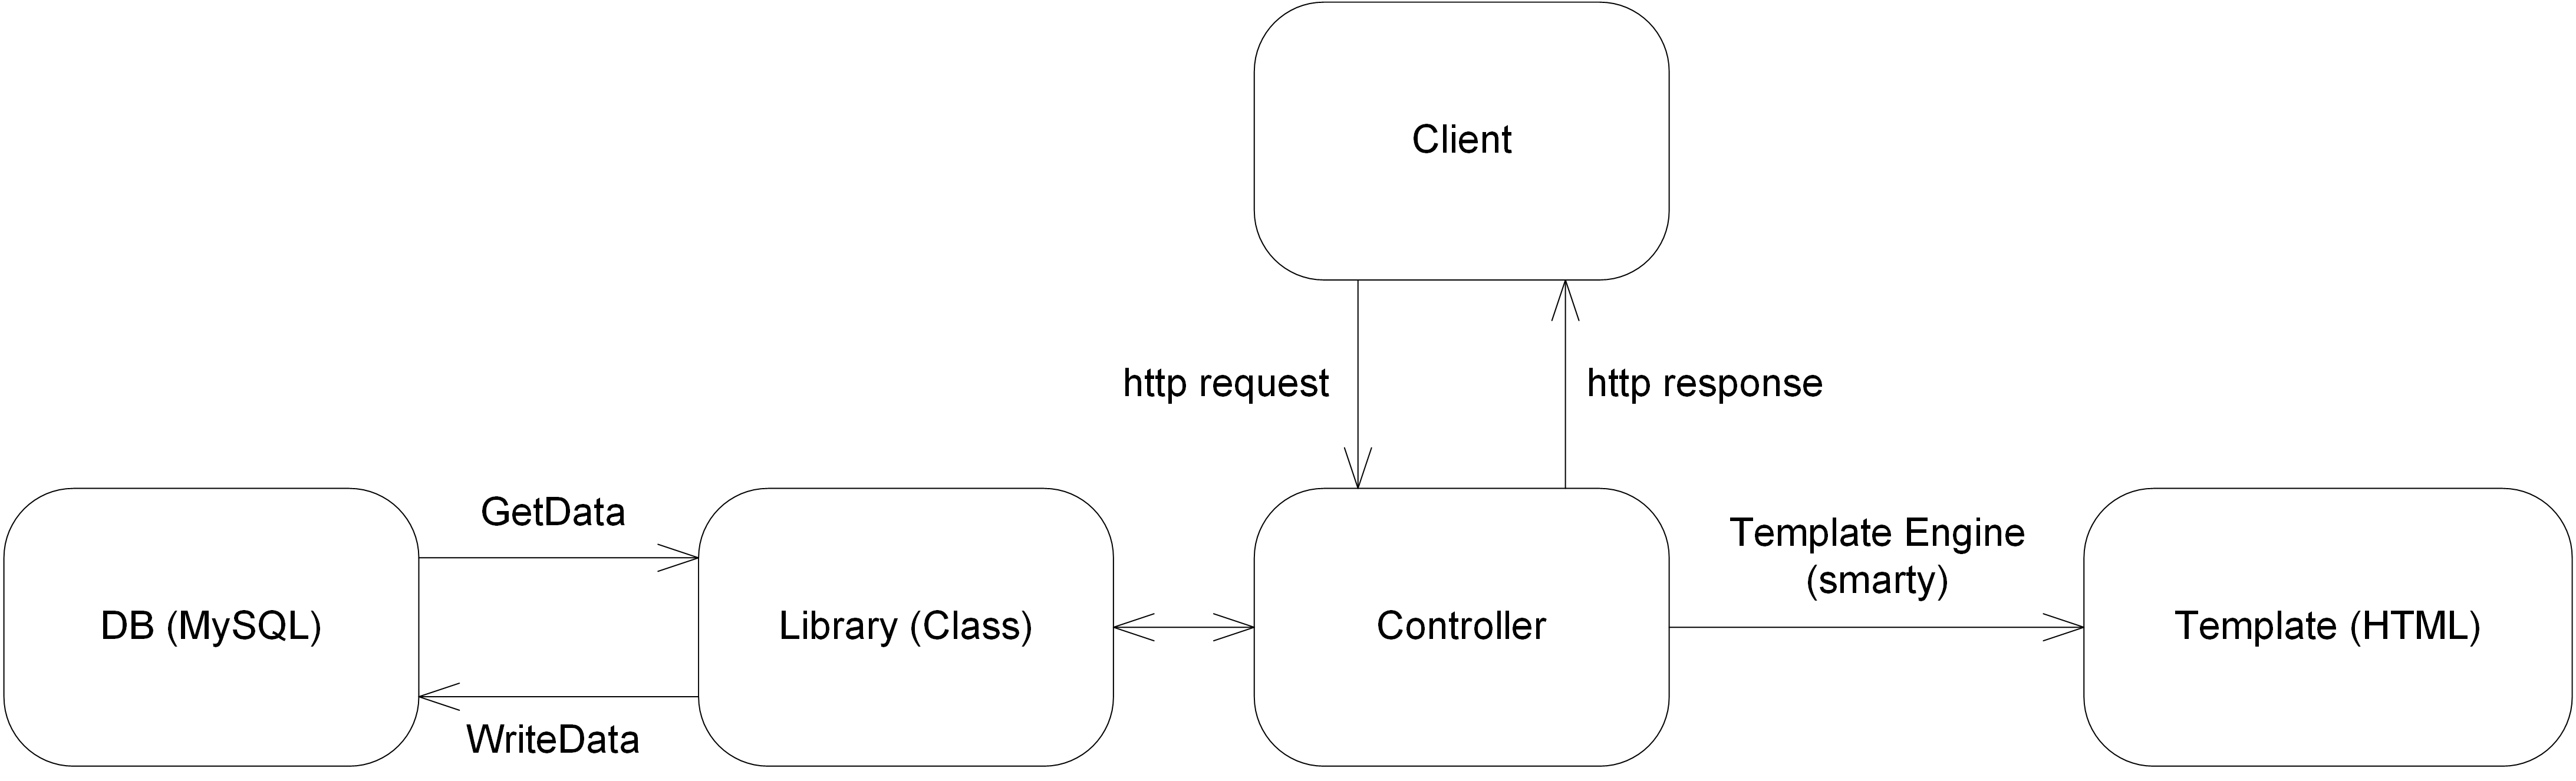
\includegraphics[width=.9\textwidth]{SoftwareArkitektur/GUI/Intro_GUI_DB/photo/webDiagram.PNG}
    \caption{Diagram over gui og databasens interaktion}
    \label{fig:web}
\end{figure}
\textbf{DB}\\
DB står for Databasen, som indeholder nogle tabeller med alle data.
\\\\
\textbf{Libary}\\
I Libary ligger der nogle klasser så det er muligt at oprette objekter, ud fra indholdet i Databasen, inde i Controlleren. 
\\\\
\textbf{Controller}\\
Controlleren indeholder alle PHP filerne som indeholder funktioner til at sætte websiden op og henter/opdaterer data fra databaserne.
\\\\
\textbf{Template}\\
Under Template ligger alle HTML filerne som strukturerer indholdet på websiden og visualiserer \glslink{gui}{gui'en}. Hertil er smarty anvendt som Template Engine, det den gør, er at det tager et PHP script, udfører det, og derefter sender forskellige genererede variabler til template (HTML filerne), hvor Smarty derefter udfører forskellige opgaver med variablerne, for til slut at kompilere skabelonen til \glslink{gui}{gui'en}.
\\\\
Til template er der også anvendt Bootstrap\footnote{http://getbootstrap.com/}, som er beregnet til at gøre webudvikling lettere, da den består af HTML- og CSS- baserede design skabeloner til typografi, formularer, knapper, navigation og andre interface komponenter, samt valgfri JavaScript udvidelser.
\\\\
For at sikre at Brugeren ikke skal opdatere websiden, hver gang de vil aflæse nogle nye data eller trykke på en af knapperne er der blevet anvendt nogle jQuery AJAX metoder, som kan bruges til at udveksle data med en server og opdatere dele af en webside uden at genindlæse hele siden.

\subsection{Database}
FlexPMS databasen er blevet anvendt til at opbevare indtastede data omkring kar og sensorøerne med deres ventil og vandingsstatus, samt aflæste værdier fra de forskellige sensorer, hvor denne database kan tilgås via \glslink{gui}{gui'en}. MySQL er databaseformatet der er valgt, og valget bunder i at denne har alle de kvaliteter systembeskrivelsen og kravspecifikationen foreskriver. Desuden er softwaren til etablering af en sådan server gratis, veldokumenteret og nem at gå til.
\\\\
Databasen indeholder nogle forskellig tabeller som er bestemt ud fra de krav vi skulle tilfredsstilles i kravspecifikation og det design der er lavet i systemarkitekturen. Disse tabeller, deres kolonnenavne og deres datatype er illustreret i figur \ref{fig:DB}. 

\begin{figure}[H]
    \centering
    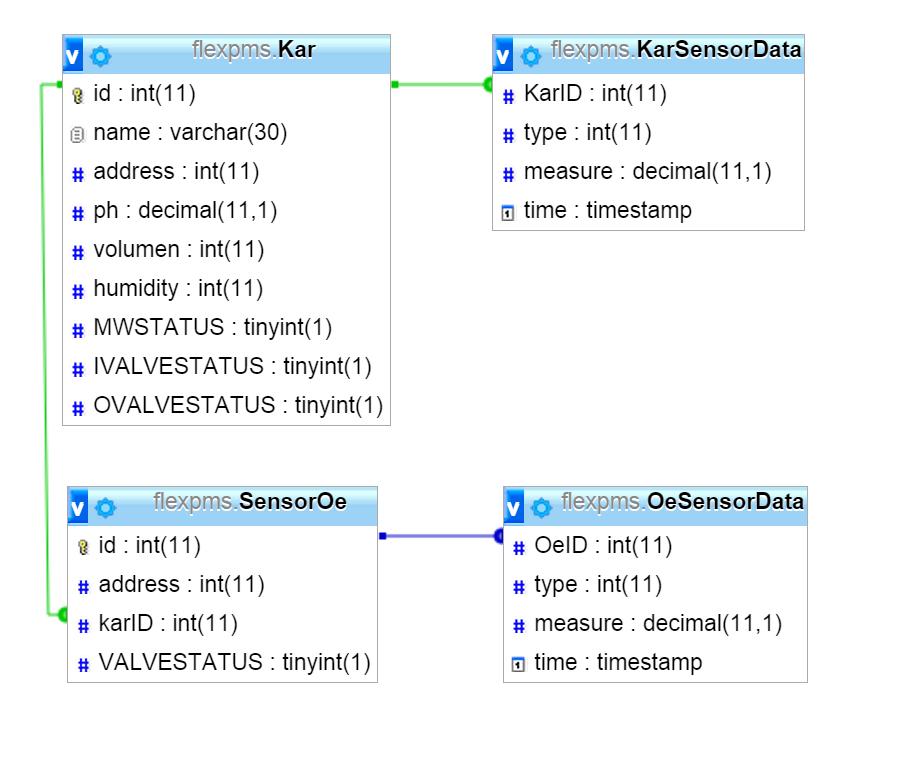
\includegraphics[width=0.7\textwidth]{SoftwareArkitektur/GUI/Intro_GUI_DB/photo/DB_diagram.PNG}
    \caption{Diagram over FlexPMS databasen}
    \label{fig:DB}
\end{figure}

Som det fremgår af diagrammet kender tabellerne til hinanden, det gør de via deres id. Hver \gls{sensoroe} og \gls{kar} har et unikt id for at sikre man kan differentiere mellem dem. Grunden til at dette er vigtigt er fordi at det sikre at data ikke bliver dubleret, ført forkert ind i tabellerne, eller har nogle forkerte interaktioner.
\\\\
En kort beskrivelse af tabellerne og deres kolonner i databasen følger:

\subsubsection{Kar}
Kar indeholder alle kar, deres kar data, som brugeren har oprettet og status for dens ventiler. Alle kar har et navn og adresse med de data som Brugeren ønsker at karet skal have. Kolonnenavnene er beskrevet i tabel \ref{table:kar_kol}.

\begin{table}[H]
\center
\setlength{\tabcolsep}{16pt}
\renewcommand{\arraystretch}{1.5}
	\begin{tabular}{ | >{\raggedright}p{2.5cm} | >{\raggedright\arraybackslash}p{9.5cm} | }
    \hline
    \rowcolor{lightgray} 
 	\textbf{Kolonnenavn} 				& \textbf{Beskrivelse} 	\\ \hline
    \textit{id} 						& Et unikt id for hver kar tabellen indeholder   						\\ \hline
   	\textit{name} 						& Navnet på karet   													\\ \hline
   	\textit{adresse}	 				& Adressen til karet    												\\ \hline
   	\textit{ph} 						& Den indtastede pH-værdi som Brugeren ønsker    						\\ \hline
   	\textit{volumen} 					& Det vandniveau/antal liter vand som Brugeren ønsker i karet 			\\ \hline
   	\textit{humidity} 					& Den jordfugtighed brugeren ønsker ved \glslink{sensoroe}{Sensor Øerne}\\ \hline
   	\vskip 4pt \textit{MWSTATUS} 		& \vskip 1px
											\begin{minipage}{9cm}
   												Status for manuel vanding:	
    											\begin{itemize}
   													\item 1: Manuel vanding er startet
   													\item 0: Manuel vanding er stoppet
   												\end{itemize}
   												\vskip 1px
 											\end{minipage}   													\\ \hline
 	\vskip 4pt \textit{IVALVESTATUS} 		& \vskip 1px 
											\begin{minipage}{9cm}
   												Status for indløbsventil:	
    											\begin{itemize}
   													\item 1: Indløbsventilen er åben
   													\item 0: Indløbsventilen er lukket
   												\end{itemize}
   												\vskip 1px
 											\end{minipage}   													\\ \hline
 	\vskip 4pt \textit{OVALVESTATUS} 		& \vskip 1px 
											\begin{minipage}{9cm}
   												Status for afløbsventil:	
    											\begin{itemize}
   													\item 1: Afløbsventilen er åben
   													\item 0: Afløbsventilen er lukket
   												\end{itemize}
   												\vskip 1px
 											\end{minipage}   
 																												\\ \hline
\end{tabular}
\caption{Beskrivelser af kolonnenavne for tabellen Kar}
\label{table:kar_kol}
\end{table}


\subsubsection{SensorOe} 
SensorOe indeholder alle Sensor Øer, deres data brugeren har oprette og status for dens ventil. hver Sensor Ø har også et KarID så man kan se hvilket Kar de hører til. Kolonnenavnene er beskrevet i tabel \ref{table:SensorOe_kol}.
\begin{table}[H]
\center
\setlength{\tabcolsep}{16pt}
\renewcommand{\arraystretch}{1.5}
	\begin{tabular}{ | >{\raggedright}p{2.5cm} | >{\raggedright\arraybackslash}p{9.5cm} | }
    \hline
    \rowcolor{lightgray} 
    \textbf{Kolonnenavn} 				& \textbf{Beskrivelse}  						\\ \hline
    \textit{id} 						& Et unikt id for hver Sensor Ø tabellen indeholder   					\\ \hline
   	\textit{adresse} 					& Adressen til Sensor Ø    													\\ \hline
   	\textit{KarID}	 					& En reference til det Kars id som Sensor Øen sidder på   				\\ \hline
   	\vskip 4pt \textit{VALVESTATUS} 	& \vskip 1px
											\begin{minipage}{9cm}
   												Status ventilen ved Sensor Øen:	
    											\begin{itemize}
   													\item 1: Ventilen er åben
   													\item 0: Ventilen er lukket
   												\end{itemize}
   												\vskip 1px
 											\end{minipage}   													\\ \hline
\end{tabular}
\caption{Beskrivelser af kolonnenavne for tabellen SensorOe}
\label{table:SensorOe_kol}
\end{table}


\subsubsection{KarSensorData}
KarSensorData indholder alle de målte værdier ved hver kar, derfor har de et KarID, som man kan se hvilken værdi det tilhører. Her indikerer type hvilken slags måling det er, hvor measure værdien der bliver målt. Ydermere er der time der angiver tiden hvor de tilhørende data blev sat ind, på den måde kan man altid tilgå de nyeste data. Kolonnenavnene er beskrevet i tabel \ref{table:karSensorData_kol}.
\begin{table}[H]
\center
\setlength{\tabcolsep}{16pt}
\renewcommand{\arraystretch}{1.5}
	\begin{tabular}{ | >{\raggedright}p{2.5cm} | >{\raggedright\arraybackslash}p{9.5cm} | }
    \hline
    \rowcolor{lightgray} 
    \textbf{Kolonnenavn} 				& \textbf{Beskrivelse}  						\\ \hline
    \textit{KarID} 						& En reference til det Kars id der bliver målt på    					\\ \hline
    \vskip 4pt \textit{type} 			& \vskip 1px
											\begin{minipage}{9cm}
   												Hvilken type sensor der er lavet måling på:	
    											\begin{itemize}
   													\item 1: pH-værdi på væsken i karret
   													\item 2: Vandniveau/Antal liter der bliver tilført til karet
   													\item 9: Gennemsnittet af jordfugtigheden målt ved Sensor Øerne 
   												\end{itemize}
   												\vskip 1px
 											\end{minipage}   													\\ \hline
   	\textit{measure} 					& Den aflæste sensor værdi 												\\ \hline
   	\textit{time}	 					& Tidspunktet værdien blev sat in i tabelen				 				\\ \hline
\end{tabular}
\caption{Beskrivelser af kolonnenavne for tabellen KarSensorData}
\label{table:karSensorData_kol}
\end{table}


\subsubsection{OeSensorData}
OeSensorData minder meget om KarSensorData men indholder alle de målte værdier ved hver \gls{sensoroe} og derfor har de et OeID. Kolonnenavnene er beskrevet i tabel \ref{table:oeSensorData_kol}.

\begin{table}[H]
\center
\setlength{\tabcolsep}{16pt}
\renewcommand{\arraystretch}{1.5}
	\begin{tabular}{ | >{\raggedright}p{2.5cm} | >{\raggedright\arraybackslash}p{9.5cm} | }
    \hline
    \rowcolor{lightgray} 
    \textbf{Kolonnenavn} 				& \textbf{Beskrivelse}  						\\ \hline
    \textit{OeID} 						& En reference til det Sensor Øs id der bliver målt på    				\\ \hline
    \vskip 4pt \textit{type} 			& \vskip 1px
											\begin{minipage}{9cm}
   												Hvilken type sensor der er lavet måling på:	
    											\begin{itemize}
   													\item 9: Jordfugtigheden målt ved Sensor Øen 
   												\end{itemize}
   												\vskip 1px
 											\end{minipage}   													\\ \hline
   	\textit{measure} 					& Den aflæste sensor værdi 												\\ \hline
   	\textit{time}	 					& Tidspunktet værdien blev sat in i tabelen				 				\\ \hline
\end{tabular}
\caption{Beskrivelser af kolonnenavne for tabellen KarSensorData}
\label{table:oeSensorData_kol}
\end{table}

\subsection{Klassediagram og metodebeskrivelse}
Ud fra implementeringen er der genereret illustrerende klassediagrammer som kan ses på figur \ref{fig:GUI_KD}, disse klasser ligger under Libary, som kan ses på figur \ref{fig:web}, klasserne er anvendt til at kunne oprette objekter, både ud fra indholdet i databasen og til at lave en Socket klient. Hvis der ønskes yderligere indsigt i hvordan specifik kode er skrevet henvises der til sourcekoden\footnote{Se bilag under Software\textbackslash www\textbackslash lib}.

\begin{figure}[H]
    \centering
    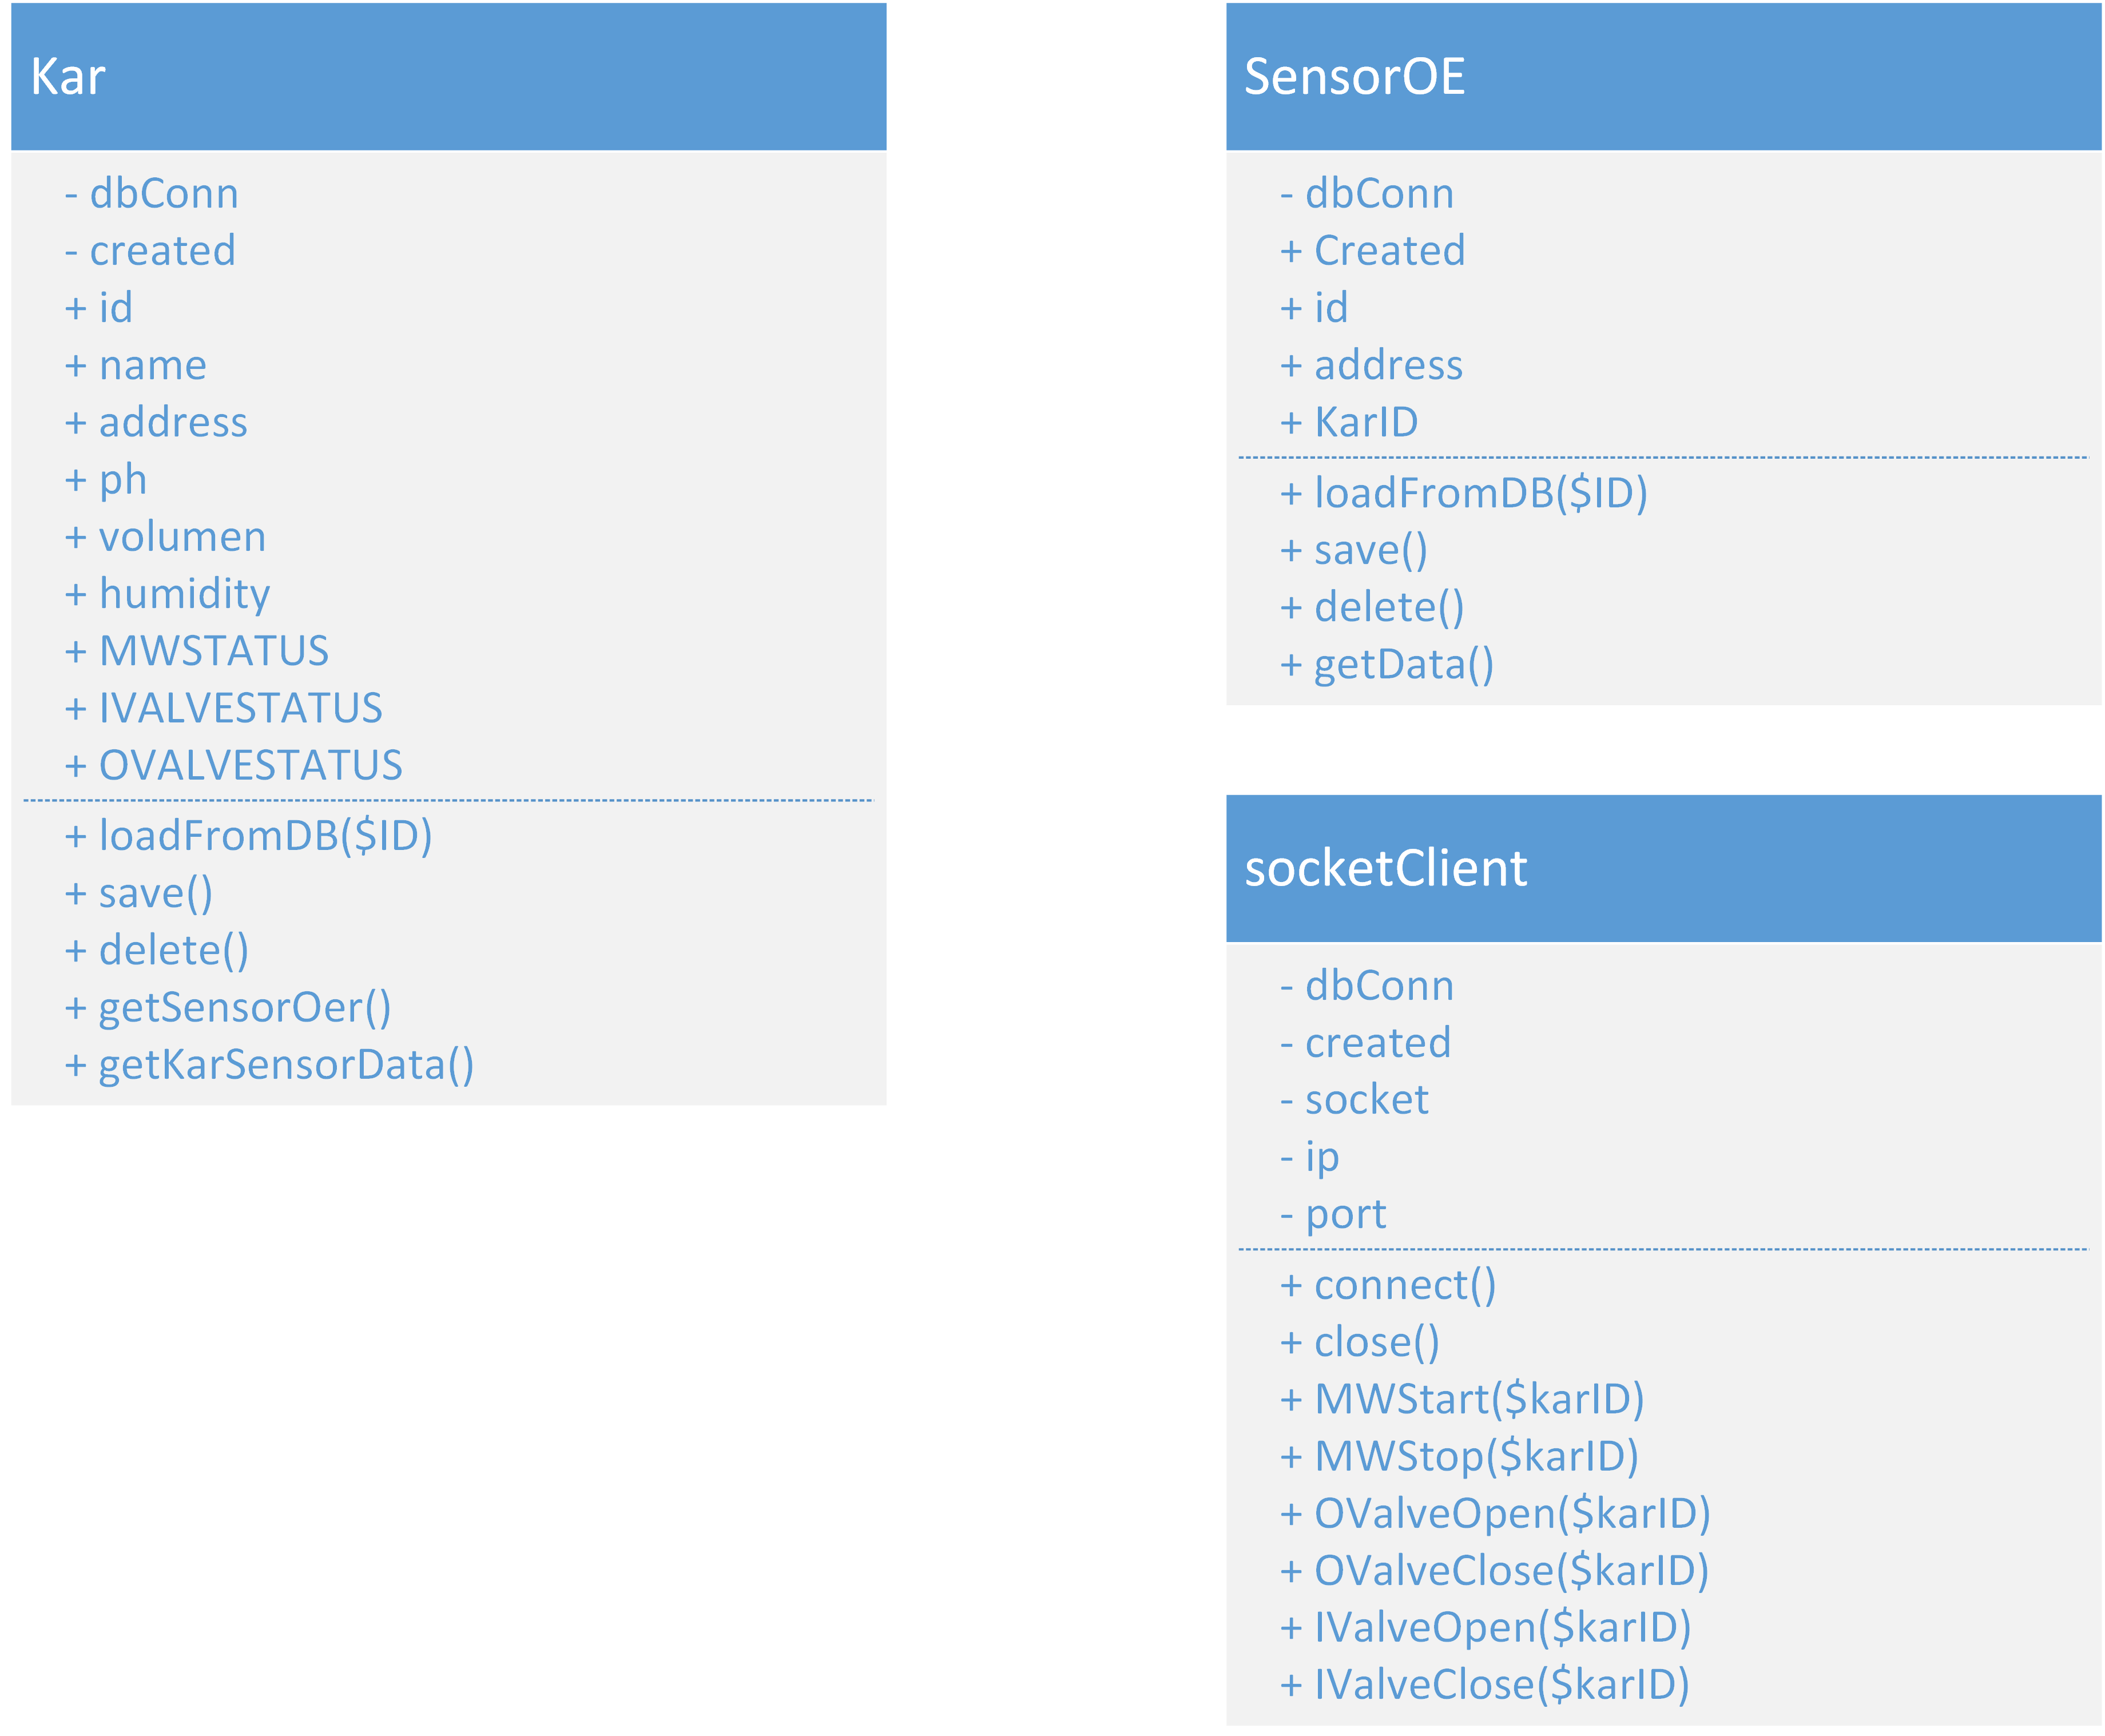
\includegraphics[width=0.7\textwidth]{SoftwareArkitektur/GUI/KlasseDiagram/photo/klasseDiagram_gui.PNG}
    \caption{Klassediagram for GUI}
    \label{fig:GUI_KD}
\end{figure}

Her kan man se der ikke er nogle forbindelse mellem de tre klasser, og det skyldes at de får alt deres information om de andre klasser gennem databasen.
 
\subsubsection{Kar klassen}
Kar klassen er en klasse, der giver mulighed for at tilgå et kar fra databasen og få alt dens information baseret på dens ID. Via klassens metoder kan de forskellige data i databasen blive redigeret, karet kan blive oprettet/slettet og man kan se hvilke \glslink{sensoroe}{Sensor Øer} der sider på karet. Den har følgende metoder:

\subsubsection{SensorOe klassen}
SensorOe klassen er en klasse, der giver mulighed for tilgå en Sensor Ø fra databasen og få alt dens information baseret på dens ID. Via klassens metoder kan de forskellige data i databasen blive redigeret, Sensor Øen kan blive oprettet/slettet og man kan se hvilket kar Sensir Øen tilhører. Den har følgende metoder:

\subsubsection{SocketClient klassen}
SocketClient klassen er en socket klient der anvendes til at sende beskeder direkte til FlexPMS, for at give besked om nogle ting systemet skal gøre. Den har følgende metoder:

\subsection{Controller}
Som de kan ses på figur \ref{fig:web}, er der en Controller, den indeholder alle PHP filer. Disse filer indeholder funktionen der anvendes til at sætte websiden op og hente/opdaterer data fra databasen. De følgende filer har hver deres opgave og disse vil blive beskrevet i følgende afsnit. Controller har følgende filerne som kan ses i tabel \ref{table:con_fil}. Hvis man ønsker at se filerne skal man gå ind under sourcekoden\footnote{Se bilag under Software\textbackslash www}.

\begin{table}[H]
\center
\setlength{\tabcolsep}{16pt}
\renewcommand{\arraystretch}{1.5}
	\begin{tabular}{ | >{\raggedright}p{3cm} | >{\raggedright\arraybackslash}p{9cm} | }
    \hline
    \rowcolor{lightgray} 
    \textbf{Kolonnenavn} 				& \textbf{Beskrivelse}  						\\ \hline
    \textit{mysql.php} 							& Opretter forbindelse til databasen											\\ \hline
    \textit{index.php}							& Bygger index/home siden til AVS												\\ \hline
    \textit{kar.php}							& Bygger kar siden til det kar man tilgår										\\ \hline
    \textit{create.php} 						& Opretter et kar, som bliver visualiseret i GUI'en og sat ind i databasen		\\ \hline
  	\textit{createSO.php} 						& Opretter en Sensor Ø som bliver visualiseret i GUI'en og sat ind i databasen	\\ \hline
   	\textit{delete.php} 						& Sletter et kar, både fra databasen og GUI'en									\\ \hline
   	\textit{deleteS.php}	 					& Sletter en Sensor Ø, både fra databasen og GUI'en							 	\\ \hline
   	\textit{edit.php}							& Redigere navnet på karet														\\ \hline
   	\textit{updateData.php}						& Opdaterer de indtastede data i karet											\\ \hline
   	\textit{auto\_refresh\_kar.php}				& opdaterer de aflæste date og er sammentidlig en fil der bliver opdateret hvert sekund \\ \hline
\end{tabular}
\caption{Beskrivelser af php filer under Controller}
\label{table:con_fil}
\end{table}
I følgende er der nogle af filerne der bliver beskrevet mere detaljeret, for at illustrer hvordan de påvirker gui'en og databasen.


\subsubsection{index}
Under template mappen ligger der en \textit{index.html} fil, som visualiserer vores webside for \gls{AVS}, denne side indeholder alle kar, men da html kun er front og antallet af kar er ukendte er der lavet noget php kode til at hente alle kar og deres informationerne hver gang man opdaterer siden, . her er smarty anvendt så man kan lave en lykke i html som så viser alle kar.\\\\
\begin{minipage}{.5\textwidth}
\begin{lstlisting}[caption=index.php]
	.
	.
	.
	.
// Get all Kar
$kars = getKars($conn);

// Render page
$smarty = new Smarty;
$smarty->assign('kars', $kars);
	.
	.
	.
	.
	.
\end{lstlisting}
\end{minipage}% This must go next to `\end{minipage}`
\begin{minipage}{.5\textwidth}
\begin{lstlisting}[caption=index.html]
	.
	.
{foreach $kars as $kar}
	<li class="list-group-item">
	<div class="row">
		<div class="col-xs-4">
			<a href="kar.php?id={$kar.id}">
				{$kar.name}
			</a>
		</div>
	.
	.																		
{/foreach}
	.
	.
\end{lstlisting}
\end{minipage}

Det gør at denne liste kan blive genereret ud fra databasen så man kan tilgå alle kar, disse kar linker til en ny side, som er baseret på karets id, se figur \ref{fig:index}. 
\begin{figure}[H]
    \centering
    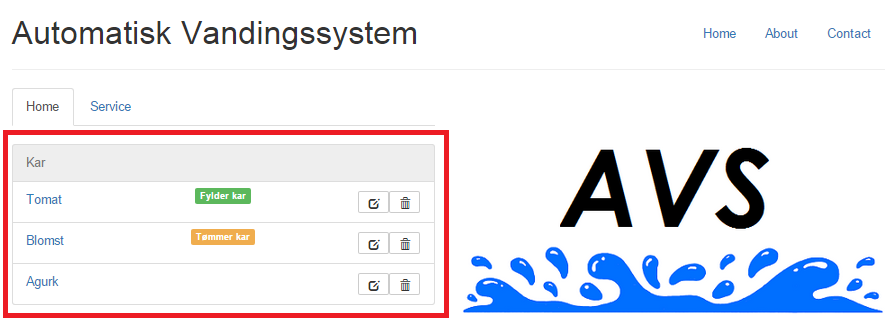
\includegraphics[width=0.9\textwidth]{SoftwareArkitektur/GUI/Controller/photo/index.PNG}
    \caption{AVS websiden}
    \label{fig:index}
\end{figure}

\subsubsection{kar}
Under template mappen ligger der en \textit{kar.html} fil, som visualisere websiden for hver enkle kar, baseret på deres id. den laver også en liste over Sensor Øerne, ved at anvende samme teknik som da man skulle have listen over kar, se figur \ref{fig:so}.  

\begin{figure}[H]
    \centering
    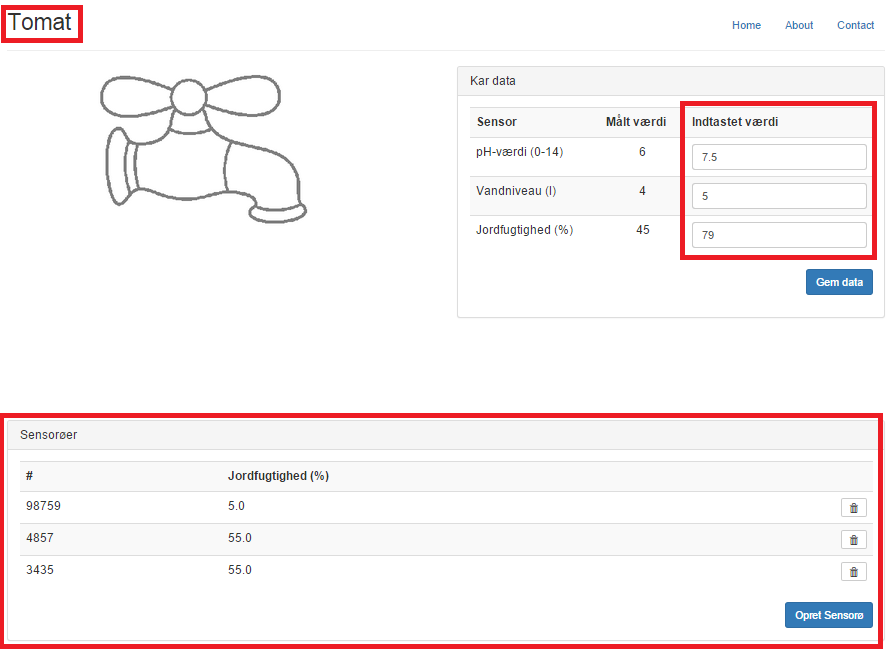
\includegraphics[width=0.9\textwidth]{SoftwareArkitektur/GUI/Controller/photo/so.PNG}
    \caption{Del af kar siden, for karet med navn Tomat}
    \label{fig:so}
\end{figure}

Desuden er der nogle knapper, som kalder en funktion så snart de bliver trykket på. Knapperne er på karet personlige side, som set på figur \ref{fig:knap}
\begin{figure}[H]
    \centering
    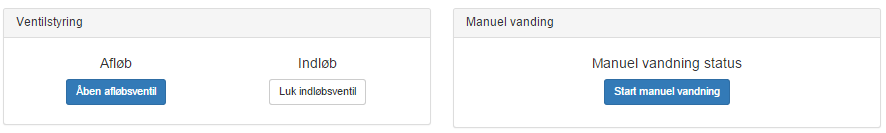
\includegraphics[width=0.9\textwidth]{SoftwareArkitektur/GUI/Controller/photo/knap.PNG}
    \caption{knapper til karet}
    \label{fig:knap}
\end{figure}

For at give et eksempel på hvordan de kalder en funktion ser vi på start manuel vanding. Den knap har php kode

\begin{lstlisting}[caption=index.php]
	.
	.
$id = $_POST['id'];
	.
	.
if(array_key_exists('MWSTART',$_POST)){
    $client->connect();
	//Manual watering start
	$client -> MWStart($id);
} 
	.
	.
\end{lstlisting}

Hvis koden til html filen har navnet 'MWSTART', og knappen bliver trykket ned, bliver der oprettet forbindelse til socket serveren og den få en besked om at manuel vanding skal startes. Knappens navn og udsende bliver sat alt efter hvilken status manuel vanding har, og den status kan aflæses på karets informationer fra databasen.


\subsubsection{auto\_refresh\_kar} 
Som nævnt tidligere er der anvendt jQuery AJAX metoder, som kan bruges til at udveksle data med en server og opdatere dele af en webside uden at genindlæse hele siden. Dette er lavet så de aflæste data bliver opdateret hvert 5 sekund og knapperenes status bliver opdateret hvert sekund. Da dette er lavet over de ting der er markeret på figur \ref{fig:auto}.  

\begin{figure}[H]
    \centering
    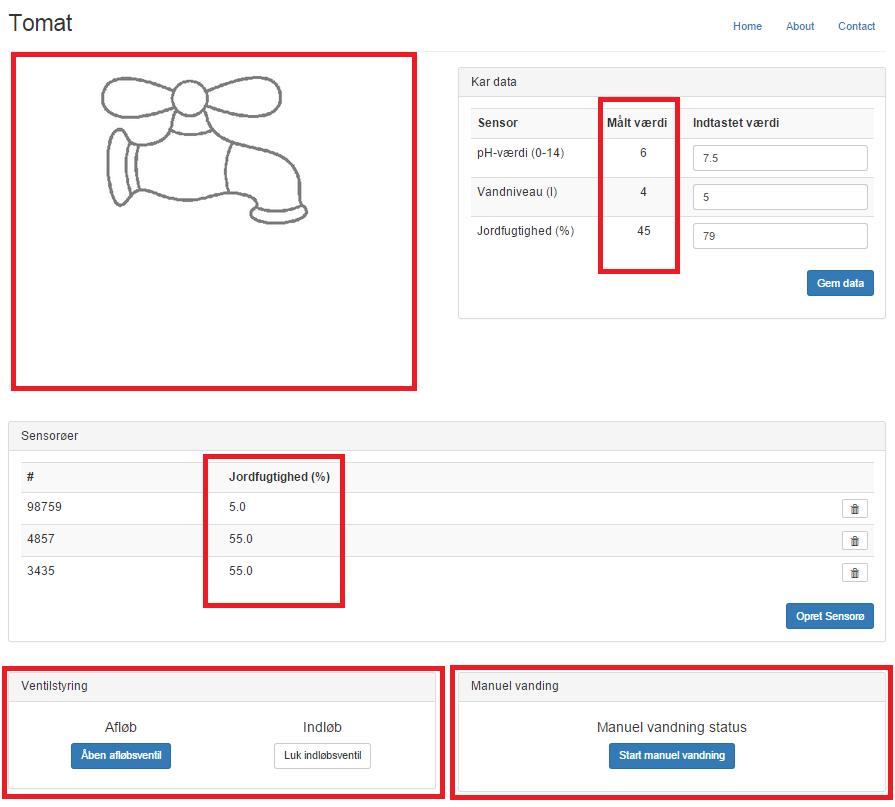
\includegraphics[width=0.9\textwidth]{SoftwareArkitektur/GUI/Controller/photo/auto.PNG}
    \caption{Dele auto\_refresh\_kar påvirker}
    \label{fig:auto}
\end{figure}

Da det går meget igen hvordan koden er implementeret for at opdaterer knapperne og de forskellige data, bliver det kun gennemgået for knappen manuel vanding. Selve processen for at få manuel vandingsstatus kan ses på følgende sekvens diagram.

\begin{figure}[H]
    \centering
    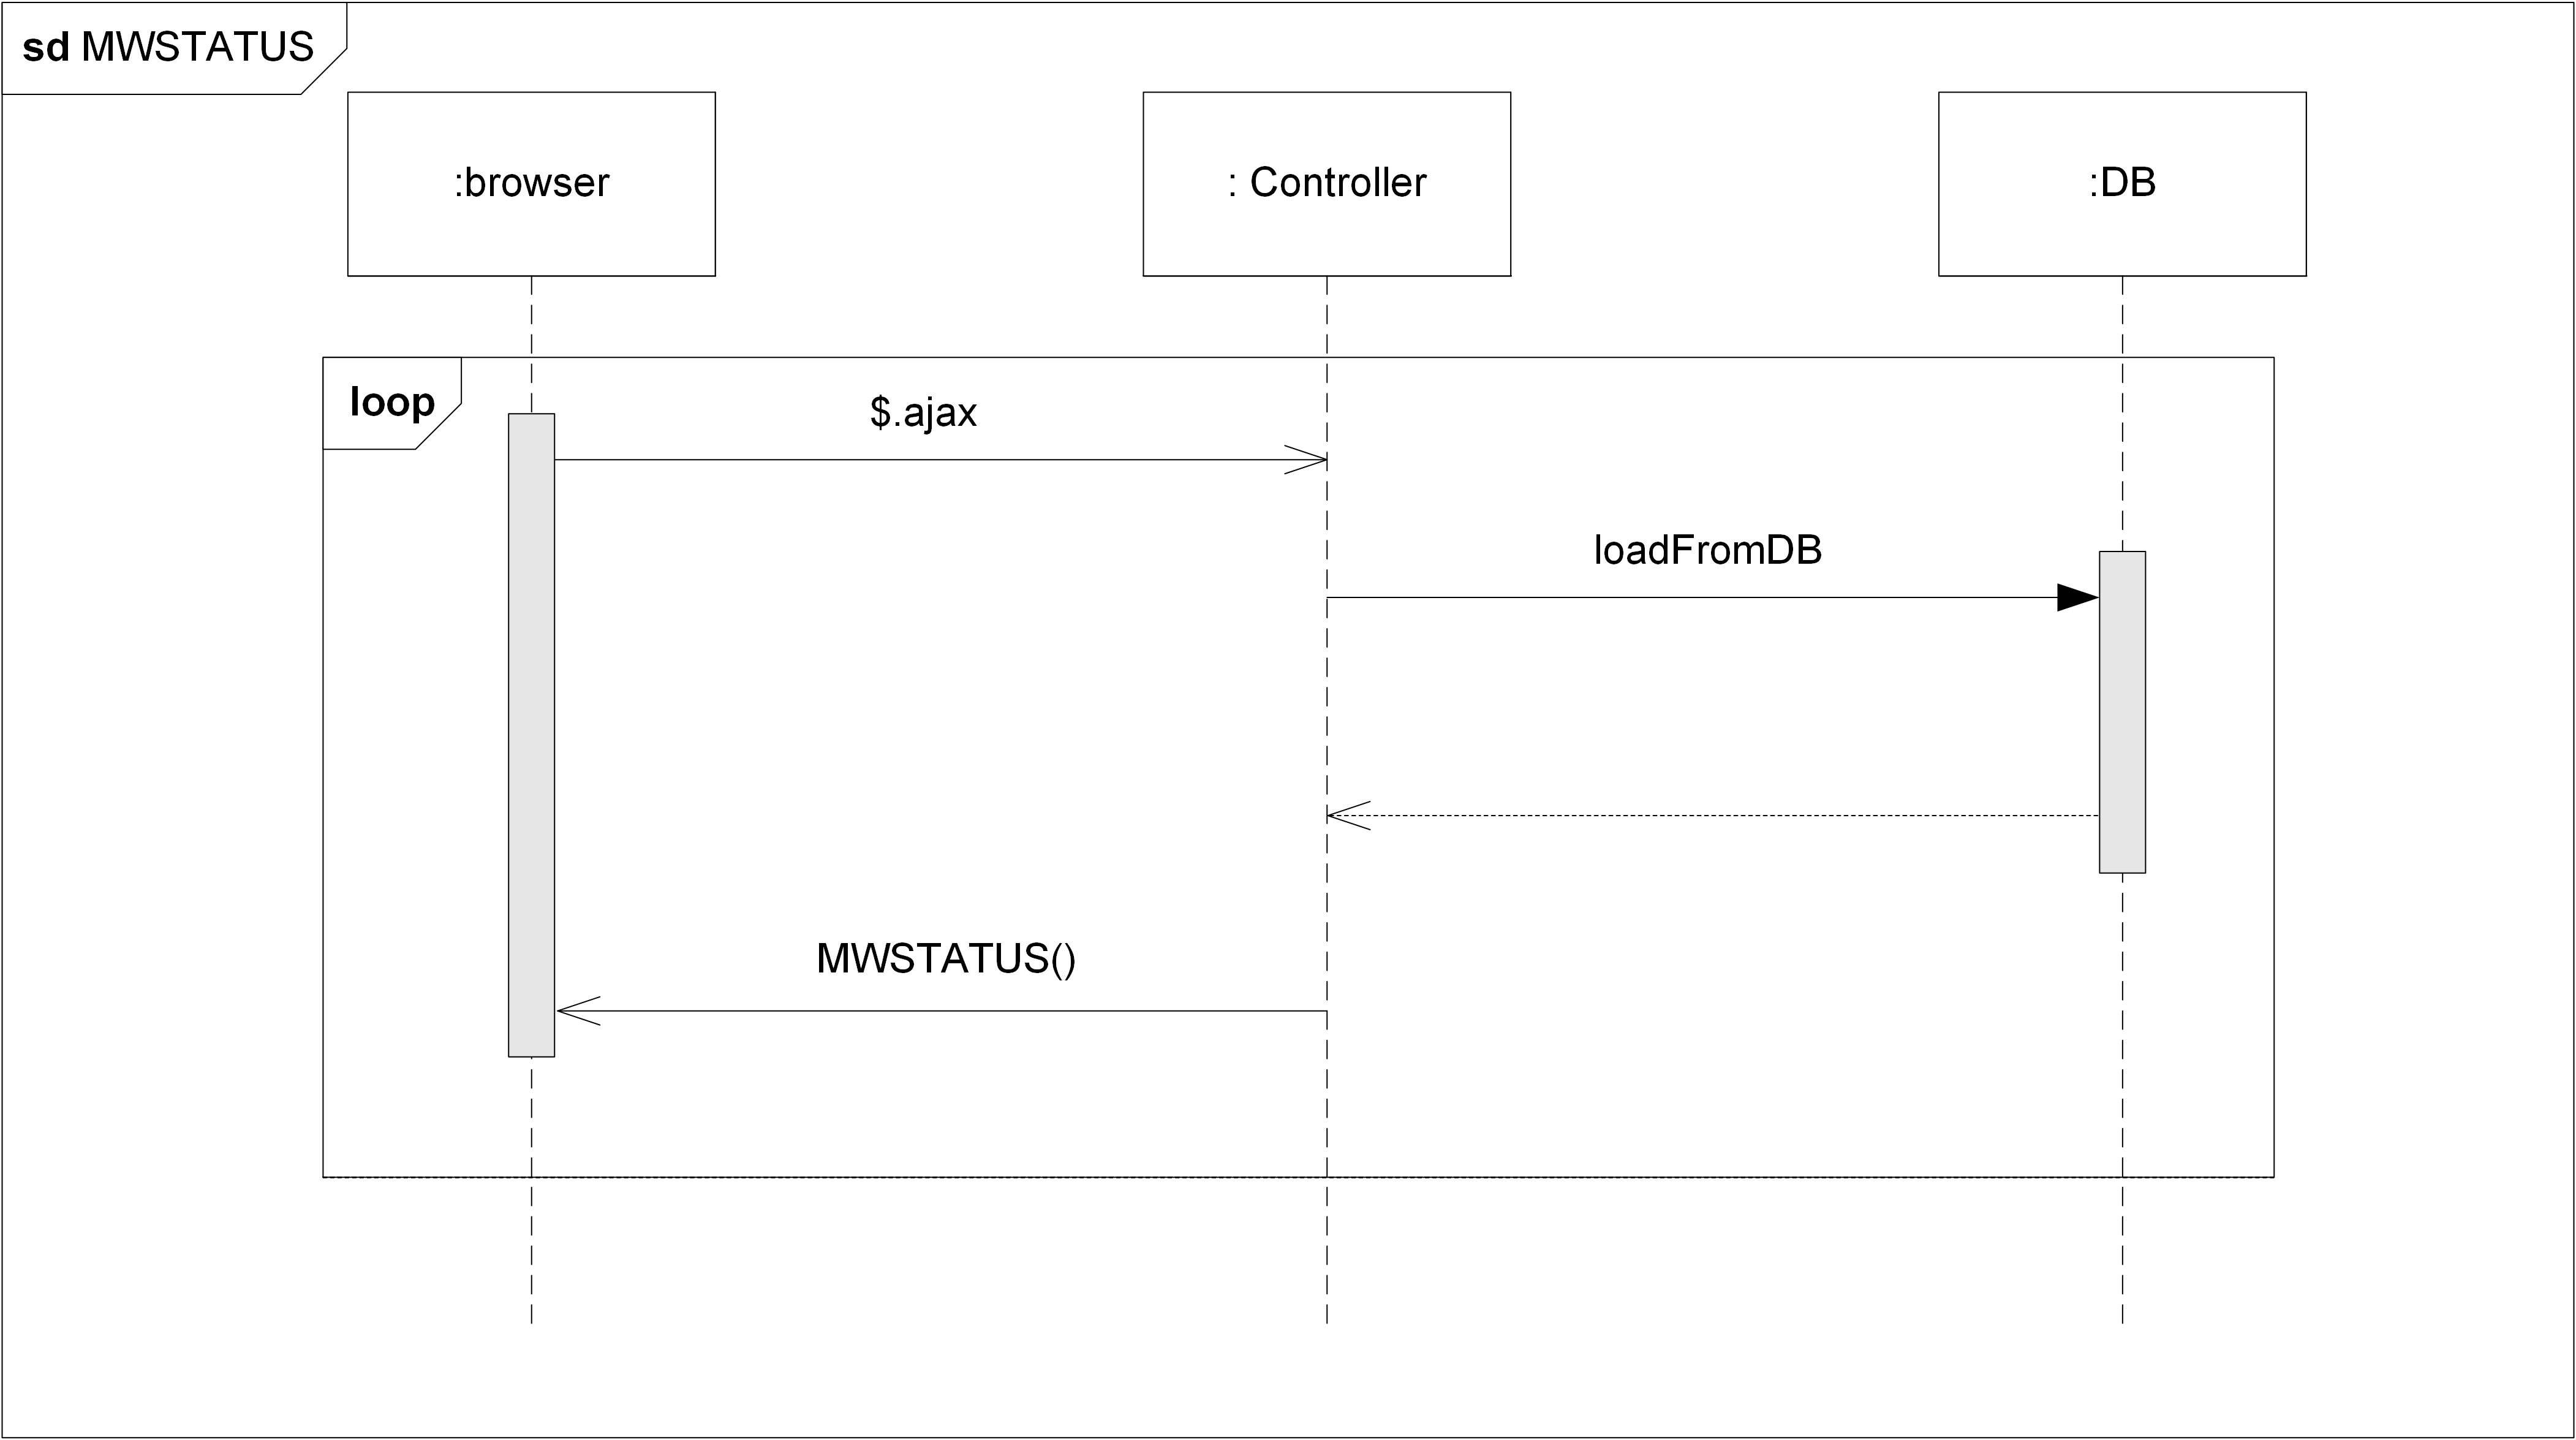
\includegraphics[width=0.8\textwidth]{SoftwareArkitektur/GUI/Controller/photo/sd_mwstatus.PNG}
    \caption{Sekvensdiagram for manuel vanding status}
    \label{fig:knap}
\end{figure}


sekvens diagrammet illustrerer, at ved at bruge ajax kan man lave et loop det sender en request hvert sekund og modtager en ønskede data. Koden for manuel vandings knappen er implementeret med JavaScript, html og php således: \\
\begin{minipage}{.5\textwidth}
\begin{lstlisting}[caption=JavaScript]
	.
	.
	.
function refreshStatuses(){
$.ajax({
  url: "auto_refresh_kar.php",
  method: "GET",
  data: { id: {$kar->id} },
  dataType: "json",
  success: function( data ) {
	if(data.mwstatus == 1){
	  $("#MWSTATUS" )
	  .html("Stop manuel vandning")
	  .removeClass('btn btn-primary btn-md')
	  .addClass('btn btn-default btn-md')
	  .attr("name","MWSTOP");
	  $("#image").attr("src","medie/VHV.png");
	}else{
	  $("#MWSTATUS" )
	  .html("Start manuel vandning")
	  .removeClass('btn btn-default btn-md')
	  .addClass('btn btn-primary btn-md')
	  .attr("name","MWSTART");
	  $("#image").attr("src","medie/VH.png");
	}
		.
		.
		.	
			
  }
 })
}
		.
		.
		.
	
$(function() {							
  refreshStatuses();
  refreshKarSensorData();
  setInterval(refreshStatuses, 1000); 		
  setInterval(refreshKarSensorData, 5000);	
});
	.
	.
	.
\end{lstlisting}
\end{minipage}% This must go next to `\end{minipage}`
\begin{minipage}{.5\textwidth}
\begin{lstlisting}[caption=html]
	.
	.
<div class="panel-body text-center">
  <h4> Manuel vandning status</h4>
  <form action="kar.php?id={$kar->id}" method="post">
    <button id="MWSTATUS" type="submit" name="" value="1" class=""></button>
  </form>
</div>
	.
	.
\end{lstlisting}
\begin{lstlisting}[caption=php]
	.
	.
$id = $_GET['id'];

// Kar connection
$kar = new Kar($conn);

// Load kar with $id
if(!$kar->loadFromDB($id))
{
	die("Ikke fundet!");
}
	.
	.
$statusses = array(
	'mwstatus' => (int) $kar->MWSTATUS,
	'ivalvestatus' => (int) $kar->IVALVESTATUS,
	'ovalvestatus' => (int) $kar->OVALVESTATUS,
	'ph' => (double) $ph,
	'volumen' => (int) $volumen,
	'humidity' => (int) $humidity,
	'sensorOeData' => $soData,
);
	
	
json_encode($statusses);
	.
	.
	.
\end{lstlisting}
\end{minipage}

I javaScript koden, bliver funktion på linje 37-42, kaldt hver gang siden bliver opdateret. og derefter bliver funktionerne knappernes status opdateret hvert sekund og kar sensor dataene bliver opdateret hvert 5 sekund. 
\\\\
På linje 4-32 bliver de funktionen der opdatere knapperne implementeret, den bruger GET metoden. Den tager det tilhørende kar id, som bliver defineret i linje 3 i php koden. 
\\\\
Id'et bliver lavet til at finde de værdier der er til karet med tilhørende kar id. derefter bliver de gemt i et array (linje 15-23), hvor den bliver lavet til en JSON repræsentation af værdien på linje 26. 
\\\
Tilbage til javaScript koden, kan værdierne fra array nu anvendes. På linje 11 bliver det undersøgt om manuel vanding er i gang og hvis det er tilfældet bliver alt koden på linje 12-17 kørt. 
\\\\
på linje 12 i javaScript koden tager vi fat i det html kode der har id "MWSTATUS", som kan ses på linje 6 i html koden. her bliver "name", "class" og teksten sat alt efter hvad manuel vandings status er. 
\\\\
Så i tilfælde af at en starter manuel vanding, bliver dens status ændret i databasen og knappen bliver opdateret uden brugeren skal genopfriske siden. 



 


\section{FlexPMS}
Lorem ipsum dolor sit amet, consectetur adipiscing elit. Vivamus at erat blandit, vehicula mauris ac, pulvinar ipsum. Nam lobortis neque libero, eget aliquam enim convallis eget. Nunc semper ex faucibus lectus pulvinar, ac molestie ligula vestibulum. Vivamus sagittis massa vitae arcu aliquam scelerisque. Vivamus in dignissim erat. Donec vitae malesuada lorem. Maecenas laoreet pharetra lobortis. Donec ac iaculis metus. Suspendisse potenti. Curabitur tincidunt risus non dui fringilla tincidunt. Fusce dui quam, bibendum non velit nec, gravida sagittis nisi. Maecenas dictum neque sit amet enim pulvinar, ac congue dolor feugiat. Etiam in felis viverra, ultricies justo id, consectetur nisl. Ut sed augue in lacus ullamcorper cursus eget sit amet turpis.\\

\PakkeDiagram{0.82}{FlexPMS}{FlexPMS}

\subsection{Kar Kommunikation}
Kar kommunikations pakken er ansvarlig for at sende beskeder til kar styringen den står altså for grænsefalden ud til sensor og aktautore igennem kommunikation til kar styringen. Den består af 3 klasser der er illustreret  i diagrammet herunder:

\KlasseDiagram{0.82}{FlexPMS}{KarBus}

\subsubsection{KarBus klassen}
Den klasse interfacer med resten af flexpms igennem den event baserede kommunikation der driver systemet klassen har således sin egen message kø og tilsvarende event handlers. KarBus har også en RS485 instans og en Protokol instans i sig, Protokol klassen er implementeringen af Karbus protokollen som KarBus klassen bruger til at sende beskeder til karret, RS485 klassen er ikke direkte brugt af KarBus.


\subsubsection{funktions beskrivelser}
\funk{void eHandleKarReady(MKarReady* msg)}{Denne eventhandler kalder den relavante funktion i protokol klassen og stykker det relavante svar sammen hvis der bliver returneret et svar fra RS485 bussen}{ingenting}
{
\funkArg{msg}{En besked om at tjekke at karret er klar til kommunikation}
}

\funk{void eHandleKarGetSensorData(MKarGetSensorData* msg)}{Denne eventhandler kalder den relavante funktion i protokol klassen og stykker det relavante svar sammen hvis der bliver returneret et svar fra RS485 bussen}{ingenting}
{
\funkArg{msg}{En besked om at hente sensor data fra karret}
}

\funk{void eHandleKarSetPumpState(MKarSetPumpState* msg)}{Denne eventhandler kalder den relavante funktion i protokol klassen og stykker det relavante svar sammen hvis der bliver returneret et svar fra RS485 bussen}{ingenting}
{
\funkArg{msg}{En besked om at styre pumpen så denne køre med den hastighed der er indehold i beskeden}
}

\funk{void eHandleKarSetPumpState(MKarSetPumpState* msg)}{Denne eventhandler kalder den relavante funktion i protokol klassen og stykker det relavante svar sammen hvis der bliver returneret et svar fra RS485 bussen}{ingenting}
{
\funkArg{msg}{En besked om at styre pumpen så denne køre med den hastighed der er indehold i beskeden}
}

\funk{void eHandleOeGetSensorData(MOeGetSensorData* msg)}{Denne eventhandler kalder den relavante funktion i protokol klassen og stykker det relavante svar sammen hvis der bliver returneret et svar fra RS485 bussen}{ingenting}
{
\funkArg{msg}{En besked om hente data fra sensor'øen}
}

\funk{void eHandleOeSetValve(MOeSetValveSate* msg)}{Denne eventhandler kalder den relavante funktion i protokol klassen og stykker det relavante svar sammen hvis der bliver returneret et svar fra RS485 bussen}{ingenting}
{
\funkArg{msg}{En besked at styre ventilen på sensor'øen}
}

\funk{void eHandleOeGetSensorType(MOeGetSensorType* msg)}{Denne eventhandler kalder den relavante funktion i protokol klassen og stykker det relavante svar sammen hvis der bliver returneret et svar fra RS485 bussen}{ingenting}
{
\funkArg{msg}{En besked at få afvide hvilken sensortype der er koblet til en bestemt adresse}
}

\funk{void eHandleKarSetValve(MKarSetValveState* msg)}{Denne eventhandler kalder den relavante funktion i protokol klassen og stykker det relavante svar sammen hvis der bliver returneret et svar fra RS485 bussen}{ingenting}
{
\funkArg{msg}{En besked at styre ventilen på karret den kan indeholde om det er afløb eller indløb der skal styres}
}

\funk{void eHandleKarGetOeList(MKarGetOeLIst* msg)}{Denne eventhandler kalder den relavante funktion i protokol klassen og stykker det relavante svar sammen hvis der bliver returneret et svar fra RS485 bussen}{ingenting}
{
\funkArg{msg}{En besked om at få en list af ø'er der er tilkoblet et kar}
}

\funk{void eHandleKarOpretOe(MKarSetOpretOe* msg)}{Denne eventhandler kalder den relavante funktion i protokol klassen og stykker det relavante svar sammen hvis der bliver returneret et svar fra RS485 bussen}{ingenting}
{
\funkArg{msg}{En besked om at oprette en ø der bliver knyttet til et kar}
}

\subsubsection{Protokol klassen}
Denne klasse er en direkte implementering af karbus protokollen det vil sige at den har en funktion per besked der er i protokollen det gør at det er nemt at tilføje beskeder til protokollen men også at andre dele af koden er mindre afhængige af protokollen og hvordan denne håndtere kommunikationen til hardware.
Klassen har en pointer til RS485 klassen som den bruger til at sende beskederne med, RS485 kunne for så vidt erstattes af en anden klasse hvis det var ønskeligt at kommunikere på anden vis end via RS485. 

\subsubsection{funktions beskrivelser}
\funk{bool sendAndReceive()}{Denne funktion kalder send og modtage funktionerne i RS485 klassen}{Der bliver returneret true hvis en besked blev modtaget ellers false}
{
}

\funk{bool getKarRdy(unsigned char karID, unsigned char\& karState)}{Denne funktion gør en besked klar til at forspørge om et kar er klar til kommunikation derefter venter den indtil der er modtaget en besked med \textKode{sendAndReceive} funktionen returtypen sætte alt efter om der modtages en besked}{Der bliver returneret true hvis en besked blev modtaget ellers false}
{
\funkArg{karID}{Adressen på det kar der kommunikeres med}
\funkArg{karState}{Parameter til at returnere status på kar}
}

\funk{bool getKarSensorData(unsigned char karID, unsigned char\& len, unsigned char\* data))}{Denne funktion gør en besked klar til at forspørge om at hente sensor data fra kar derefter venter den på svar fra \textKode{sendAndReceive} hvis denne returnere true tjekkes det om vi har fået det rigtige svar hvis det er tilfældet sættes de relevante svar værdier}{Der bliver returneret true hvis en besked blev modtaget ellers false}
{
\funkArg{karID}{Adressen på det kar der kommunikeres med}
\funkArg{len}{længden af det data der er modtaget}
\funkArg{data}{data'en der blev modtager lagt i et char array}
}

\funk{bool setPumpState(unsigned char karID, unsigned char\& state)}{Denne funktion gør en besked klar til at forespørge om at styre pumpen på et kar derefter venter den på svar fra \textKode{sendAndReceive} hvis denne returnere true tjekkes det om vi har fået det rigtige svar hvis det er tilfældet sættes de relevante svar værdier}{Der bliver returneret true hvis en besked blev modtaget ellers false}
{
\funkArg{karID}{Adressen på det kar der kommunikeres med}
\funkArg{state}{Bruges til at modtage hvilken state pumpen skal sættes til samt at returnere hvilken tilstand den blev sat til såfremt at vi får et rigtigt svar fra bussen}
}

\funk{bool getOeSensorData(unsigned char karID, unsigned char oeID, unsigned char\& len, unsigned char\* data)}{Denne funktion gør en besked klar til at forespørge om at hente data fra en sensorø derefter venter den på svar fra \textKode{sendAndReceive} hvis denne returnere true tjekkes det om vi har fået det rigtige svar hvis det er tilfældet sættes de relevante svar værdier}{Der bliver returneret true hvis en besked blev modtaget ellers false}
{
\funkArg{karID}{Adressen på det kar der kommunikeres med}
\funkArg{oeID}{Adressen på den ø vi øsnker at hente data fra}
\funkArg{len}{længden på svaret fra bussen, dette parameter bruges til at returnere værdier}
\funkArg{data}{den data der er indhentet fra ø'en, dette parameter bruges til at returnere værdier}
}

\funk{bool setOeValve(unsigned char karID, unsigned char oeID, unsigned char\& state)}{Denne funktion gør en besked klar til at forespørge om at styre ventil på en sensor ø der er tilkoblet et kar, derefter venter den på svar fra \textKode{sendAndReceive} hvis denne returnere true tjekkes det om vi har fået det rigtige svar hvis det er tilfældet sættes de relevante svar værdier}{Der bliver returneret true hvis en besked blev modtaget ellers false}
{
\funkArg{karID}{Adressen på det kar der kommunikeres med}
\funkArg{oeID}{Adressen på den ø vi øsnker at hente data fra}
\funkArg{state}{Bruges til at modtage hvilken state ventilen skal sættes til samt at returnere hvilken tilstand den blev sat til såfremt at vi får et rigtigt svar fra bussen}
}

\funk{bool setKarValve(unsigned char karID, unsigned char\& ventilID, unsigned char\& state)}{Denne funktion gør en besked klar til at forespørge om at styre en ventil der er tilkoblet et kar, derefter venter den på svar fra \textKode{sendAndReceive} hvis denne returnere true tjekkes det om vi har fået det rigtige svar hvis det er tilfældet sættes de relevante svar værdier}{Der bliver returneret true hvis en besked blev modtaget ellers false}
{
\funkArg{karID}{Adressen på det kar der kommunikeres med}
\funkArg{ventilID}{Adressen på den ventil der skal styres bruges også til at returnere hvilken ventil der blev styret}
\funkArg{state}{Bruges til at modtage hvilken state ventilen skal sættes til samt at returnere hvilken tilstand den blev sat til såfremt at vi får et rigtigt svar fra bussen}
}

\funk{bool getKarOelist(unsigned char karID, unsigned char\& len, unsigned char\* data)}{Denne funktion gør en besked klar til at forespørge om at få en liste af tilkoblede ø'er på kar, derefter venter den på svar fra \textKode{sendAndReceive} hvis denne returnere true tjekkes det om vi har fået det rigtige svar hvis det er tilfældet sættes de relevante svar værdier}{Der bliver returneret true hvis en besked blev modtaget ellers false}
{
\funkArg{karID}{Adressen på det kar der kommunikeres med}
\funkArg{len}{længden på svaret fra bussen, dette parameter bruges til at returnere værdier}
\funkArg{data}{den liste af ø'er der er indhentet fra karret, dette parameter bruges til at returnere værdier}
}

\funk{bool getOeSensorType(unsigned char karID, unsigned char oeID, unsigned char\& fsID)}{Denne funktion gør en besked klar til at forespørge om at få typen af en bestemt sensor, derefter venter den på svar fra \textKode{sendAndReceive} hvis denne returnere true tjekkes det om vi har fået det rigtige svar hvis det er tilfældet sættes de relevante svar værdier}{Der bliver returneret true hvis en besked blev modtaget ellers false}
{
\funkArg{karID}{Adressen på det kar der kommunikeres med}
\funkArg{oeID}{Adressen på den ø vi øsnker at hente data fra}
\funkArg{fsID}{Adressen på den sensor vi øsnker at kende typen på}
}

\funk{bool opretOeKar(unsigned char karID, unsigned char\& oeID)}{Denne funktion gør en besked klar til at forespørge om at oprette en ø på et kar, derefter venter den på svar fra \textKode{sendAndReceive} hvis denne returnere true tjekkes det om vi har fået det rigtige svar hvis det er tilfældet sættes de relevante svar værdier}{Der bliver returneret true hvis en besked blev modtaget ellers false}
{
\funkArg{karID}{Adressen på det kar der kommunikeres med}
\funkArg{oeID}{Adressen på den ø vi ønsker at oprettet}
}

\subsubsection{RS485 klassen}
Denne klasse bliver brugt til at sende og modtage data på RS485 bussen, den gør brug af termios interfacet til at skrive data ud serielt fra raspberry pi's GPIO pinde, den kan også styre en GPIO pin der fungere som transmit enable(TxEn). Dette er en nødvendighed da hardware der konvertere fra logisk signal til differentielt signal kan sættes i transmit eller receive mode. Klassen er også ansvarlig for at styre pariteten på de bytes vi sender. Grunden til dette er at KarBus bruger mark/space paritet til at indikere om den byte der sendes er en adresse eller en almindelig data byte. Dette har givet lidt udfordring i forhold til at regne pariteten ud for alle bytes der sendes da kommunikationen ellers ikke ville fungere, i linux kan der officielt kun sendes med odd eller even paritet.
Selve modtager delen er implementeret som en state machine dette er gjort for at holde styr på adresseringen.

\StateDiagram{0.82}{FlexPMS}{RS485RX}

\subsubsection{funktions beskrivelser}

\funk
{void initGPIO()}
{Denne funktion initiere GPIO'en der skal bruges som TxEn}
{ingen}
{
}

\funk
{void txEnable(bool state)}
{Denne funktion bruges til at tænde og slukke for TxEn}
{ingen}
{
\funkArg{state}{Kan være true for at tænde txen eller false for at slukke}
}

\funk
{void sendChar(char ch, bool address)}
{Denne funktion sender en enkelt char ad gangen samtidigt vender den pariteten før den sender den holder også øje med hvilken paritet vi er efterladt i da vi skal bruge det når vi modtager}
{ingen}
{
\funkArg{ch}{Den char der skal sendes}
\funkArg{address}{Hvis denne er true indikere det at den char vi sender er en adresse ellers hvis den er false sendes der data}
}

\funk
{bool parityCheck(char \&ch, bool parity) }
{Denne funktion bruges til at checke pariteten på de char's der bliver indlæst af modtageren for at identificere om det er en adresse}
{hvilken paritet en char er blevet læst med}
{
\funkArg{ch}{Den char der skal tjekkes paritet på}
\funkArg{parity}{Kaldes med den tilstand der ønskes at tjekke paritet efter}
}

\funk
{int getChar(char \&ch, bool \&address) }
{Denne funktion bruges til at indlæse en char fra hardware der tjekkes her på paritets fejl da linux håndtere paritets fejl ved at sende \textKode{0xFF} efter fulgt af \textKode{0x00} dermed kan vi vide hvordan vi skal teste hvilken paritet char'en burde have haft}
{hvor mange bytes \textKode{read()} har indlæst}
{
\funkArg{ch}{Den char der skal tjekkes paritet på}
\funkArg{parity}{Kaldes med den tilstand der ønskes at tjekke paritet efter}
}

\funk
{void getPacket()}
{Denne funktion indeholder state machinen der bruger getChar til at indlæse char og bestemmer hvor i bufferen de skal placeres alt efter om det er en char som er en adresse eller det er en data char, den holder også øje med når vi har modtaget en hel besked det gør den via length i selve beskeden}
{intet}
{
}

\funk
{void sendPacket(char *packet, unsigned int len)}
{Denne funktion bruges til at sende en besked det er blot en for løkke der sender den char pointers værdier som funktionen for med som parametre til \textKode{sendChar()}}
{intet}
{
\funkArg{packet}{den besked der skal sendes}
\funkArg{len}{Hvor mange char's pointeren packet indeholder}
}

\funk
{bool getMessage(char* msg)}
{Denne funktion bruges til at tjekke om der er en besked klar til at blive indlæst}
{returnere true hvis der er en besked klar ellers false}
{
\funkArg{msg}{kan bruges til at læse bufferen ud}
}

\funk
{void initBuffer()}
{Denne funktion bruges til at gøre bufferen klar til at modtage en ny besked}
{intet}
{
}

\funk
{void RS485send(Bus\_Message\* txMessage)}
{Denne funktion bruges af protokollen til at sende en besked på bussen}
{intet}
{
\funkArg{txMessage}{den besked der skal sendes i stuct format}
}

\funk
{bool RS485read(Bus\_Message\* rxMessage)}
{Denne funktion bruges af protokollen til at sende en besked på bussen}
{Hvis der er modtaget en besked returneres true}
{
\funkArg{txMessage}{den besked der skal sendes i stuct format}
}




\subsection{Template}
Lorem ipsum dolor sit amet, consectetur adipiscing elit. Vivamus at erat blandit, vehicula mauris ac, pulvinar ipsum. Nam lobortis neque libero, eget aliquam enim convallis eget. Nunc semper ex faucibus lectus pulvinar, ac molestie ligula vestibulum. Vivamus sagittis massa vitae arcu aliquam scelerisque. Vivamus in dignissim erat. Donec vitae malesuada lorem. Maecenas laoreet pharetra lobortis. Donec ac iaculis metus. Suspendisse potenti. Curabitur tincidunt risus non dui fringilla tincidunt. Fusce dui quam, bibendum non velit nec, gravida sagittis nisi. Maecenas dictum neque sit amet enim pulvinar, ac congue dolor feugiat. Etiam in felis viverra, ultricies justo id, consectetur nisl. Ut sed augue in lacus \textKode{ullamcorper} cursus eget sit amet turpis.

\KlasseDiagram{0.82}{FlexPMS}{FlexPMS}

\subsubsection{Temp klassen}
Donec venenatis luctus massa, sed interdum eros interdum quis. Morbi eget massa ut ante venenatis efficitur. Praesent tempus euismod tempus. Integer ac nisl eros. Praesent faucibus nisl non faucibus tincidunt. Pellentesque habitant morbi tristique senectus et netus et malesuada fames ac turpis egestas. Aenean tristique augue libero, interdum fringilla nibh consequat vel. Nullam id dapibus velit. Fusce sit amet dolor mollis, iaculis tellus ut, cursus nisi. \textKode{Curabitur} eleifend congue lacus sit amet ullamcorper. Pellentesque mollis tincidunt lectus sit amet cursus. Aenean euismod velit tellus, non lobortis quam dapibus a.

\SekvensDiagram{0.82}{FlexPMS}{Template}

\subsubsection{funktions beskrivelser}
Duis egestas congue odio, et convallis arcu eleifend vel. Vivamus sed risus congue, tincidunt ipsum in, volutpat eros. Vestibulum eros quam, vulputate eu varius id, pellentesque at risus. Duis in iaculis dolor, consequat sollicitudin libero. Aliquam pulvinar gravida nunc vitae pulvinar. Nam ligula nisl, dapibus at facilisis vel, porttitor id metus. Curabitur malesuada enim mauris, ut dignissim sapien bibendum sit amet.


\funk{void sendChar(char Data, char addr)}
{Jeg er en funktion der sender en char til hardwaren og sørger for at vende paritet rigtigt char til hardwaren og sørger for at vende paritet rigtigt}
{ingenting}
{
\funkArg{Data}{Dette er selve den char der skal sendes-Dette er selve den char der skal sendes Dette er selve den char der skal sendes}
}



\section{Kar}

\PakkeDiagram{0.82}{Kar}{Kar}

\section{Sensor Ø}

\PakkeDiagram{0.82}{SensorOe}{SensorOe}